\documentclass{beamer}
\usepackage[english]{babel}
\usepackage{amsmath,amssymb,graphicx}

%%%%%%%%%% Start TeXmacs macros
\newcommand{\cdummy}{\cdot}
\newcommand{\mathd}{\mathrm{d}}
\newcommand{\nospace}{}
\newcommand{\tmmathbf}[1]{\ensuremath{\boldsymbol{#1}}}
\newcommand{\tmop}[1]{\ensuremath{\operatorname{#1}}}
%%%%%%%%%% End TeXmacs macros

\begin{document}

{\slideshow{\begin{frame}
  \
  
  \
  
  \
  
  \
  
  \
  
  \title{计算视觉与模式识别}
  
  \maketitle
\end{frame}

\begin{frame}
  \frametitle{透视缩减}
  
  {\hspace{4em}}\resizebox{0.7\columnwidth}{!}{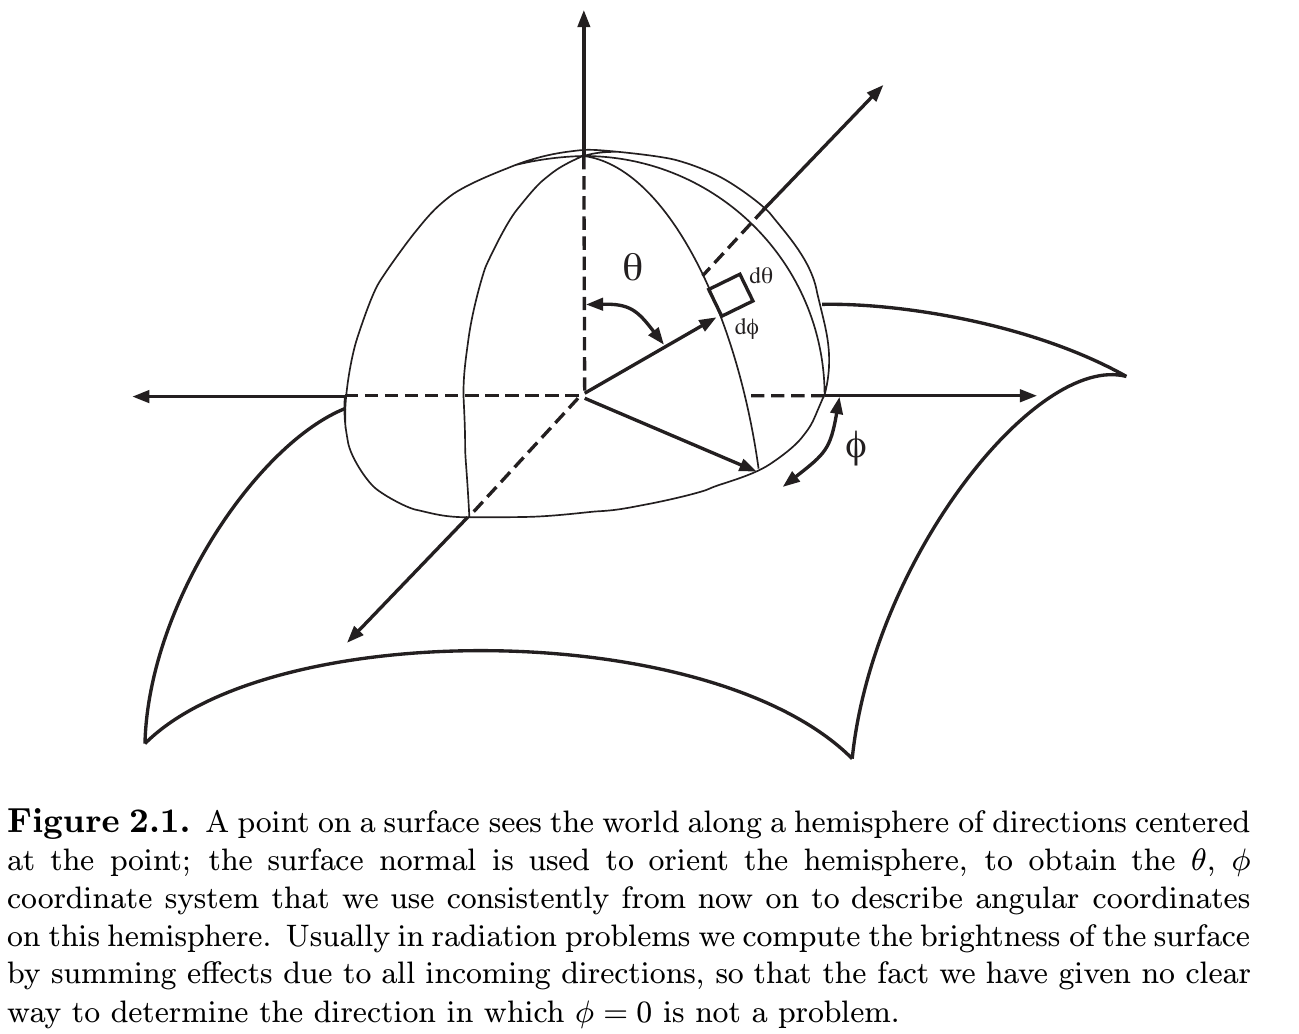
\includegraphics{img/point_on_a_surface_hemisphere.png}}
\end{frame}

\begin{frame}
  \frametitle{立体角}
  
  \
  
  {\hspace{4em}}\resizebox{0.7\columnwidth}{!}{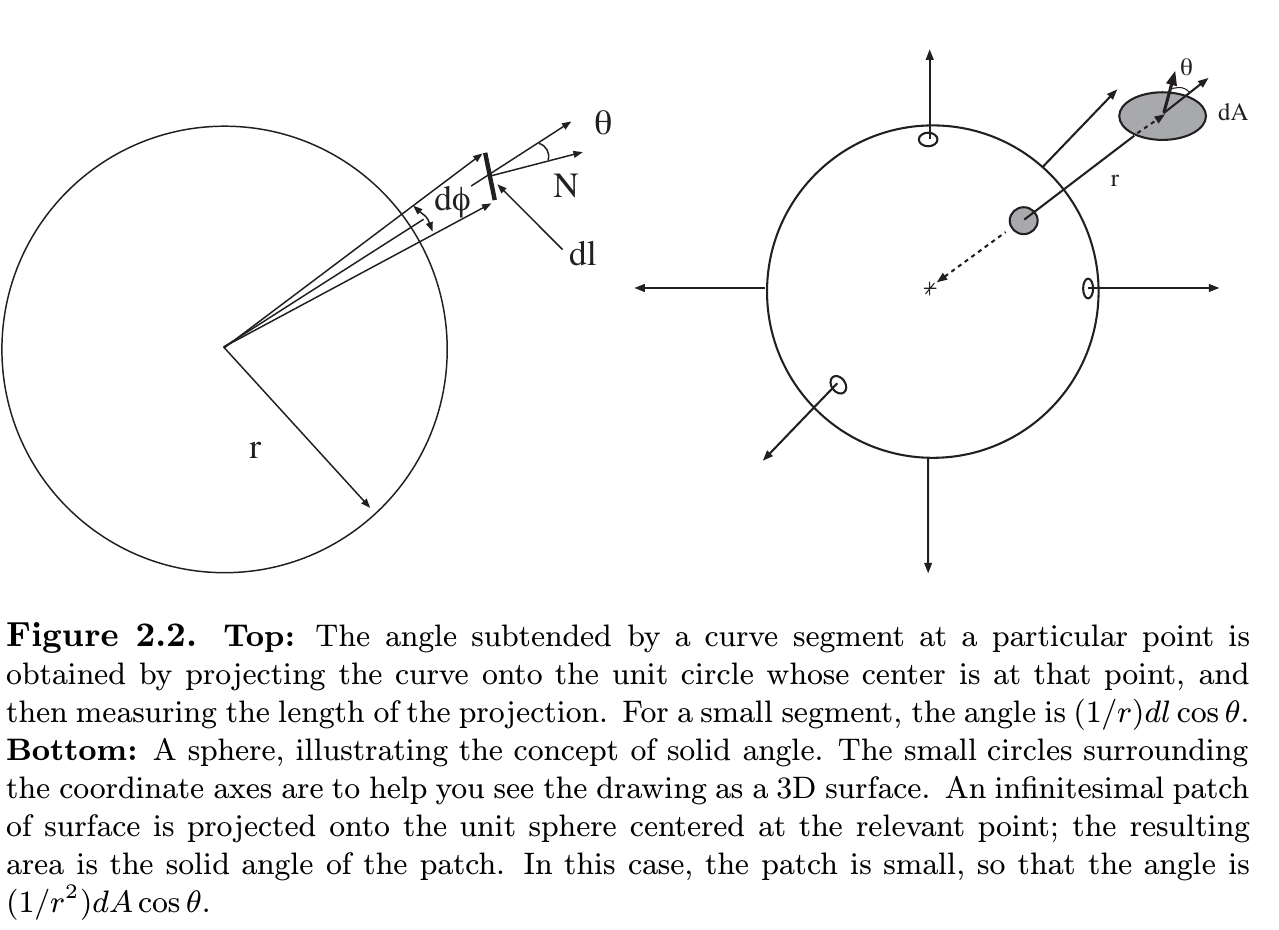
\includegraphics{img/solid_angle.png}}
\end{frame}

\begin{frame}
  \frametitle{}
  \begin{eqnarray*}
    \mathd \varphi & = & \frac{\mathd l \nospace \cos \theta}{r}\\
    \mathd \omega & = & \frac{\mathd A \nospace \cos \theta}{r^2}\\
    &  & \\
    \mathd \omega & = & \frac{r \nospace \sin \theta \mathd \varphi \cdummy r
    \mathd \theta}{r^2}\\
    & = & \nospace \sin \theta \mathd \theta \mathd \varphi
  \end{eqnarray*}
\end{frame}

\begin{frame}
  \frametitle{辐射率}
  
  {\hspace{5em}}\resizebox{!}{0.8\textheight}{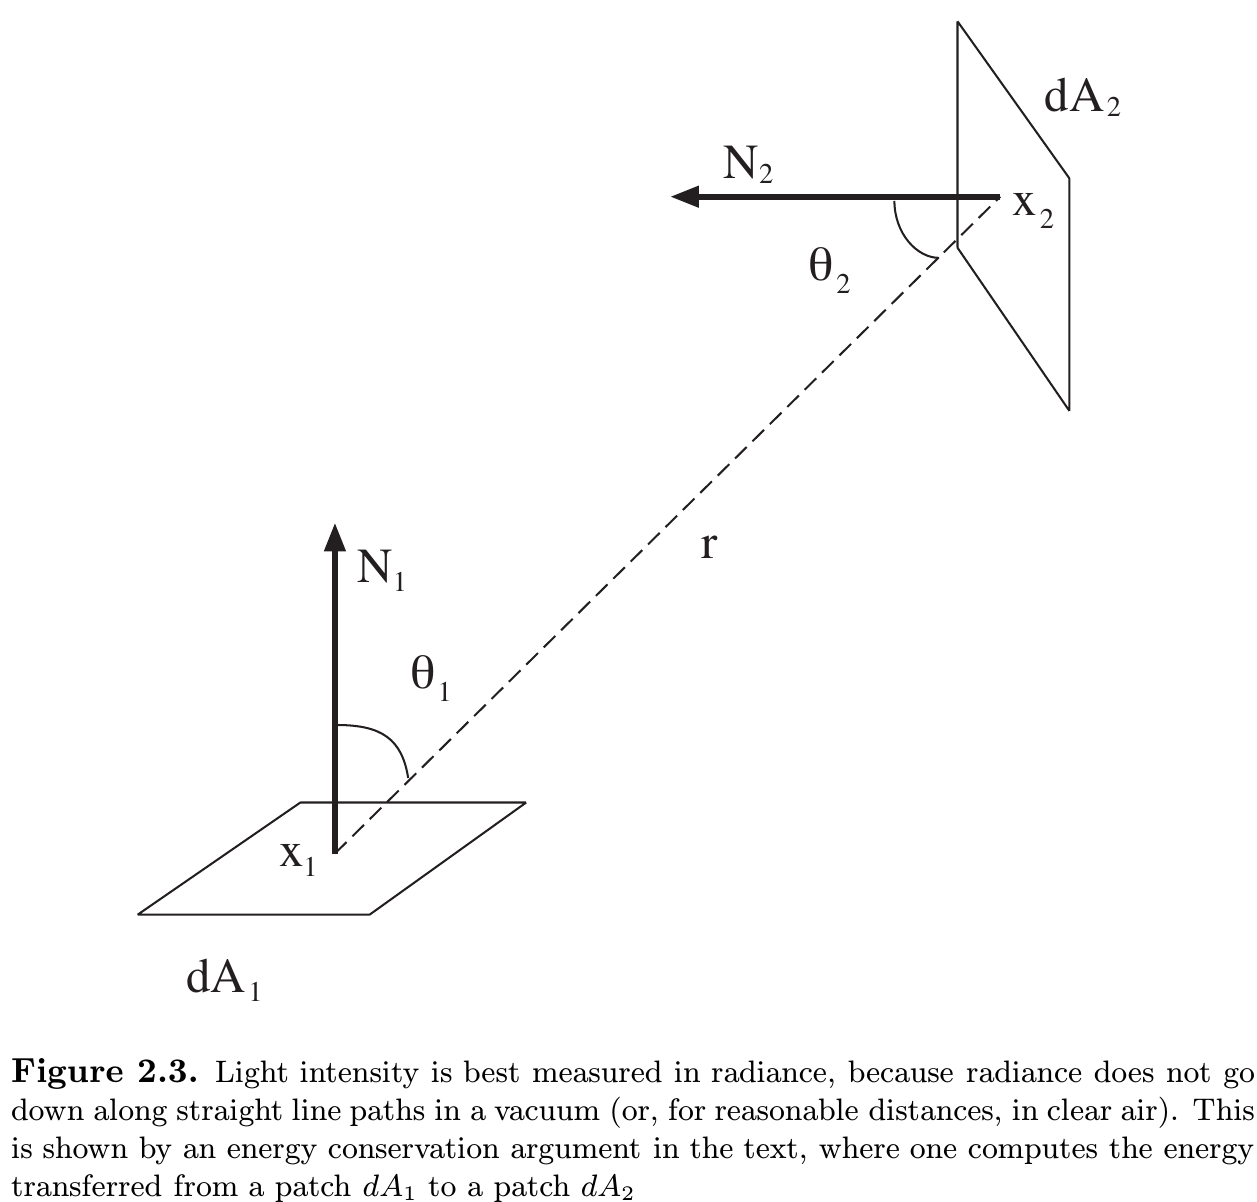
\includegraphics{img/radiance_A1_to_A2.png}}
\end{frame}

\begin{frame}
  \frametitle{}
  \[ L (x_1, \theta, \varphi) (\cos \theta_1 \mathd A_1) (d \omega) (d
     \nospace t) \]
  \begin{eqnarray*}
    \mathd^3 E_{1 \rightarrow 2} & = & L (x_1, x_1 \rightarrow x_2) \cos
    \theta_1 \mathd \omega_{2 (1)} \mathd A_1 \mathd t\\
    & = & L (x_1, x_1 \rightarrow x_2) \frac{\cos \theta_1 \cos \theta_2
    \mathd A_2 \mathd A_1 \mathd t}{r^2}\\
    \mathd \omega_{2 (1)} & = & \frac{\cos \theta_2 \mathd A_2}{r^2}\\
    \mathd^3 E_{1 \rightarrow 2} & = & L (x_1, x_1 \rightarrow x_2) \cos
    \theta_2 \mathd \omega_{1 (2)} \mathd A_2 \mathd t\\
    & = & L (x_1, x_1 \rightarrow x_2) \frac{\cos \theta_2 \cos \theta_1
    \mathd A_1 \mathd A_2 \mathd t}{r^2}\\
    \mathd \omega_{1 (2)} & = & \frac{\cos \theta_1 \mathd A_1}{r^2}
  \end{eqnarray*}
\end{frame}

\begin{frame}
  \frametitle{}
  
  辐照度
  \begin{eqnarray*}
    L_i (x, \theta_i, \varphi_i) \cos \theta_i \mathd \omega &  & 
  \end{eqnarray*}
  双向反射分布函数
  \begin{eqnarray*}
    \rho_{\tmop{bd}} (\theta_o, \varphi_o, \theta_i, \varphi_i) & = &
    \frac{\mathd L_0 (x, \theta_o, \varphi_o)}{L_i (x, \theta_i, \varphi_i)
    \cos \theta_i \mathd \omega}
  \end{eqnarray*}
  
  
  \ 
\end{frame}

\begin{frame}
  \frametitle{BRDF性质}
  
  设
  \begin{eqnarray*}
    L_i (\tmmathbf{x}, \theta_i, \varphi_i) & = & \int_{\Omega} \frac{1}{\cos
    \theta} \cos \theta \mathd \omega\\
    & = & \int_0^{2 \pi} \int_0^{\frac{\pi}{2}} \sin \theta \mathd \theta
    \mathd \varphi\\
    & = & 2 \pi
  \end{eqnarray*}
  得
  \begin{eqnarray*}
    L (\tmmathbf{x}, \theta_o, \varphi_o) & = & \int_{\Omega} \rho_{\tmop{bd}}
    (\theta_o, \varphi_o, \theta_i, \varphi_i) L_i (\tmmathbf{x}, \theta_i,
    \varphi_i) \cos \theta_i \mathd \omega
  \end{eqnarray*}
\end{frame}

\begin{frame}
  \frametitle{}
  \begin{eqnarray*}
    2 \pi & \geqslant & \int_{\Omega_o} L_o (\tmmathbf{x}, \theta_o,
    \varphi_o) \cos \theta_o \mathd \omega_o\\
    & = & \int_{\Omega_o} \int_{\Omega_i} \rho_{\tmop{bd}} (\theta_o,
    \varphi_o, \theta_i, \varphi_i) L_i (\tmmathbf{x}, \theta_i, \varphi_i)
    \cos \theta_i \mathd \omega_i \cos \theta_o \mathd \omega_o\\
    & = & \int_{\Omega_o} \int_{\Omega_i} \rho_{\tmop{bd}} (\theta_o,
    \varphi_o, \theta_i, \varphi_i) \mathd \omega_i \cos \theta_o \mathd
    \omega_o\\
    & = & \int_{\Omega_o} \int_{\Omega_i} \rho_{\tmop{bd}} (\theta_o,
    \varphi_o, \theta_i, \varphi_i) \sin \theta_i \mathd \theta_i \mathd
    \varphi_i \cos \theta_o \sin \theta_o \mathd \theta_o \mathd \varphi_o
  \end{eqnarray*}
  
\end{frame}

\begin{frame}
  \frametitle{辐射度}
  \begin{eqnarray*}
    B (\tmmathbf{x}) & = & \int_{\Omega} L (\tmmathbf{x}, \theta, \varphi)
    \cos \theta \mathd \omega
  \end{eqnarray*}
  设
  \begin{eqnarray*}
    L_o (\tmmathbf{x}, \theta_o, \varphi_o) & = & L_o (\tmmathbf{x})
  \end{eqnarray*}
  \begin{eqnarray*}
    B (\tmmathbf{x}) & = & \int_{\Omega} L_o (\tmmathbf{x}) \cos \theta \mathd
    \omega\\
    & = & L_o (\tmmathbf{x}) \int_o^{\frac{\pi}{2}} \int_o^{2 \pi} \cos
    \theta \sin \theta \mathd \varphi \mathd \theta\\
    & = & \pi L_o (\tmmathbf{x})
  \end{eqnarray*}
\end{frame}

\begin{frame}
  \frametitle{方向性半球反射}
  \begin{eqnarray*}
    \rho_{\tmop{dh}} (\theta_i, \varphi_i) & = & \frac{\int_{\Omega} L_o
    (\tmmathbf{x}, \theta_o, \varphi_o) \cos \theta_o \mathd \omega_o}{L_i
    (\tmmathbf{x}, \theta_i, \varphi_i) \cos \theta_i \mathd \omega_i}\\
    & = & \int_{\Omega} \frac{L_o (\tmmathbf{x}, \theta_o, \varphi_o)}{L_i
    (\tmmathbf{x}, \theta_i, \varphi_i) \cos \theta_i} \cos \theta_o \mathd
    \omega_o\\
    & = & \int_{\Omega} \rho_{\tmop{bd}} (\theta_o, \varphi_o, \theta_i,
    \varphi_i) \cos \theta_o \mathd \omega_o
  \end{eqnarray*}
  
\end{frame}

\begin{frame}
  \frametitle{漫反射}
  
  
  \begin{eqnarray*}
    \rho_{\tmop{bd}} (\theta_o, \varphi_o, \theta_i, \varphi_i) & = & \rho\\
    \rho_d & = & \int_{\Omega} \rho_{\tmop{bd}} (\theta_o, \varphi_O,
    \theta_i, \varphi_i) \cos \theta_o \mathd \omega_o\\
    & = & \int_{\Omega} \rho \cos \theta_o \mathd \omega_o\\
    & = & \rho \int_o^{\frac{\pi}{2}} \int_o^{2 \pi} \cos \theta_o \sin
    \theta_o \mathd \theta_o \mathd \varphi_o\\
    & = & \pi \rho\\
    \rho_{\tmop{brdf}} & = & \frac{\rho_d}{\pi}
  \end{eqnarray*}
\end{frame}

\begin{frame}
  \frametitle{镜面反射}
  
  \resizebox{1\columnwidth}{!}{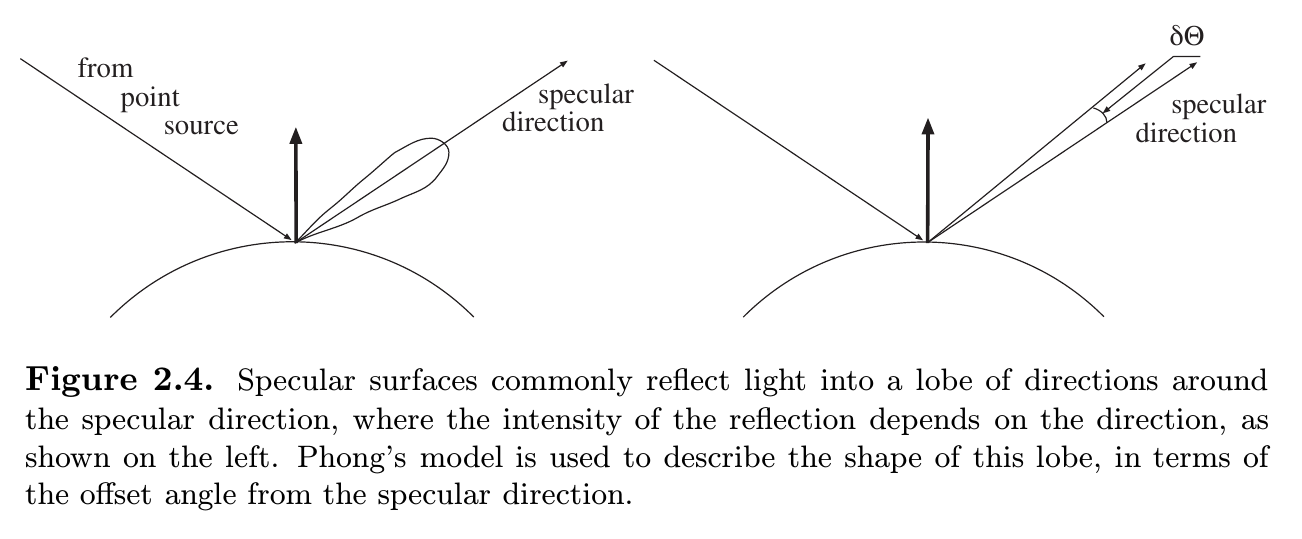
\includegraphics{img/specular_reflect.png}}
\end{frame}

\begin{frame}
  \frametitle{漫反射与镜面反射}
  
  
  \begin{eqnarray*}
    k (\delta \theta) & = & \cos^n (\delta \theta)\\
    & = & \cos^n (\theta_s - \theta_o)
  \end{eqnarray*}
  
  \begin{eqnarray*}
    L (\tmmathbf{x}, \theta_o, \varphi_o) & = & \rho_d (\tmmathbf{x})
    \int_{\Omega} L (\tmmathbf{x}, \theta_i, \varphi_i) \cos \theta_i \mathd
    \omega + \rho_s (\tmmathbf{x}) L (\tmmathbf{x}, \theta_s, \varphi_s) k
    (\delta \theta)\\
    & = & \rho_d (\tmmathbf{x}) \int_{\Omega} L (\tmmathbf{x}, \theta_i,
    \varphi_i) \cos \theta_i \mathd \omega + \rho_s (\tmmathbf{x}) L
    (\tmmathbf{x}, \theta_s, \varphi_s) \cos^n (\theta_s - \theta_o)
  \end{eqnarray*}
\end{frame}}}

\end{document}
